%!TEX root = main.tex
\chapter{Background}
\label{chap:background}
In this chapter we present the theoretical background for this thesis. This includes information on Computer-supported reflection, agile development and the notion of self-organizing teams and a teams importance in agile development. 

\section{Computer-supported reflection}
Reflection is critical to workplace learning, enabling employees to make sense of complex and dynamic situations\citep{Schon1983}. Boud et al.\citep{boudreflection1985} defined learning through reflection as: 
\begin{quote}
\emph{Those intellectual and affective activities in which individuals engage to explore their experiences in order to lead to new understandings and appreciations.}
\end{quote}
The MIRROR project\footnote{\url{http://www.mirror-project.eu/}}, describes reflective learning as:
\begin{quote}
\emph{The conscious re-evaluation of experience for the purpose of guiding future behavior, acknowledging the need to attend to feelings, ideas as well as behavior associated with work experience.}\citep{krogstiemodel}
\end{quote}

Work and reflection on this work are heavily connected\citep{Schon1983}, both driving each other forward. Experiences are created through work, and these experiences can be reflected upon. Reflection can be based on both a memory of an experience, and on data from the experience. Revisiting and reflecting on a work experience leads to a better understanding of the experience and allows for learning from it. Reflection can help developers learn from experiences and gain knowledge of how to deal with work-related challenges. This relationship between reflection and learning has been modeled as an experience-based learning cycle\citep{boudreflection1985,Korthagen_Vasalos_2005, KolbModel}. In the reflective process you return to the experience, attend to connected feelings and re-evaluate
the experience. These cycles show that the reflective process and the experience connects in order to produce an outcome.
Reflection has both individual and social dimensions,\citep{Hoeyrup_2004,Woerkom_Croon_2008}. Social wise reflection is often performed collaboratively by teams performing a joint task as organized practice, and therefore shares some common ground and experience. 

Most reflective learning in a work environment, happens analogically without support of technology\citep{Schindler_Eppler_2003}. Technology has been shown to increase the potency of reflection and reflective learning at work, meaning computer-supported reflection tools can be used to promote reflection and experience based learning \citep{krogstiereflectionwork, Lin1999}. 

\subsection{The MIRROR model}
\label{mirrorsection}
The MIRROR model of Computer Supported Reflective Learning (CSRL), is a work on how to incorporate reflection in to the daily routine at work. 
MIRROR presents a reflection-learning cycle based on the CSRL cycle in Figure \ref{csrlmodel}, which accounts for the role of technology in reflective learning at the workplace. The MIRROR CSRL model is presented in Figure \ref{mirrormodel}, and shows how tools can support the reflection process. One key part of this model is the reflection session. These sessions is where the team gathers and actively reflects on experiences, both informal or formal. The model shows that the reflective process and the experience connects in order to produce an outcome. This result with identified behavioral changes and new perspectives can then be applied to the working environment. 
\begin{figure}[!htpb]
\centering
	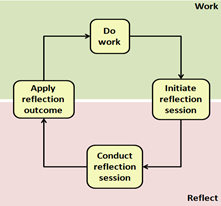
\includegraphics[width=0.8\textwidth]{csrlmodel}
\caption{CSRL Cycle view \citep{Krogstie2011}}
\label{csrlmodel}
\end{figure}

\begin{figure}[h!]
\centering
	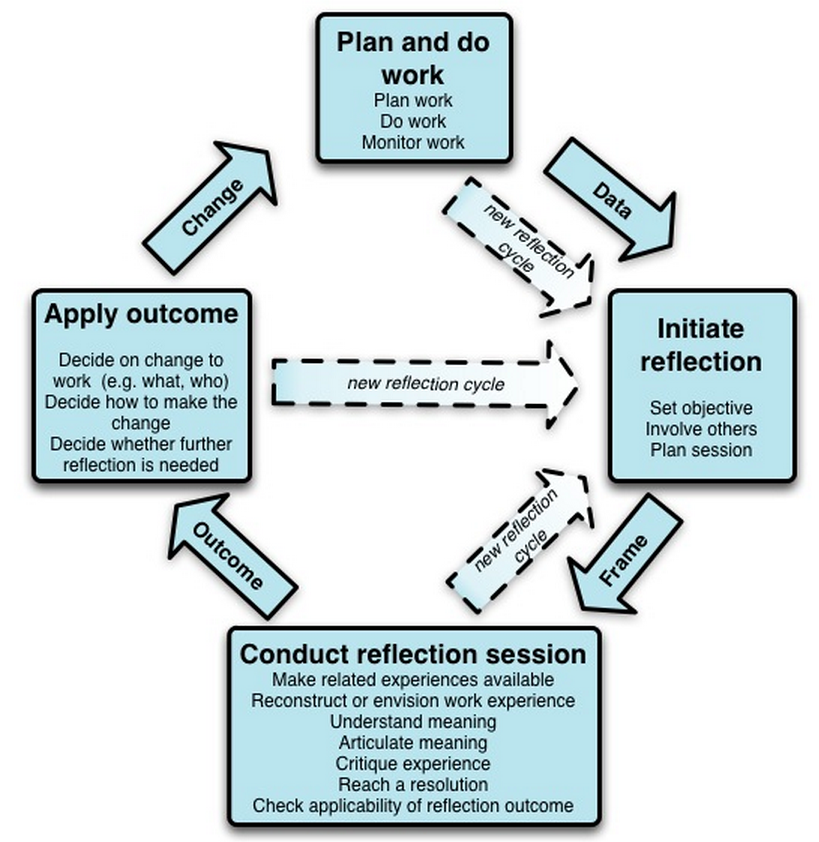
\includegraphics[width=\textwidth]{mirrorcsrl}
\caption{MIRROR CSRL model \citep{csrlmirror121}}
\label{mirrormodel}
\end{figure}

Figure \ref{mirrormodel} depicts the different stages the MIRROR-model introduces. Our thesis builds mainly on the two first phases, the \emph{Plan and do work} and \emph{Initiate reflection} phase. The application developed supports these phases during work, collecting experiences and reflection and making the results available for later use. The application also enables teams and team-members to prepare for the reflection session. Team-leaders can also initiate the reflection session, by creating a frame or a plan for the team reflection session. 
\clearpage
\subsubsection{Plan and do work}
The \emph{plan and do work} stage is any work related activity. This includes everyday work, planning and monitoring. It also includes simulated work in both real and virtual environments, and the activity can be both individual or collaborative. The data resulting from this phase can be used to reconstruct and make sense of work experiences. 

\subsubsection{Initiate reflection}
The \emph{Initiate reflection} stage is where the reflection cycle starts when reflection has been triggered. The initiation of reflection includes setting the objective for the reflection session and making a plan for it. The result of this phase is a frame to be used during the reflection session. This frame can be seen as the \emph{"setup"} of the reflection session, creating a context for the session. Such a frame allows for an efficient time-use and keeping the discussion to the topics that have been identified in the frame. 

\subsubsection{Conduct reflection session}
The \emph{Conduct reflection session} stage is the reflection session itself, and is based on the frame identified in the \emph{Initiate reflection}stage. The reflection stage will in our context feature agile software development teams in a retrospective reflection session. Activities during this stage use the identified frame to create a discussion around the experience collected by the application and use the reflection outcomes to improve work. 

\subsubsection{Apply reflection outcome}
The \emph{Apply reflection outcome} stage, is where the reflection outcomes are used to create a change in the daily work routine of the teams. This includes what to change and who will be involved in the change. How to make the change, f.ex if it can be immediately applied and if it should be recommended to other teams as well. 

We will utilize this model during both the development and evaluation of the proof-of-concept prototype. This prototype will capture experiences and store them for use in reflection sessions. This will make it easy for users to revisit the experience and reflect upon them, be it individually or collaboratively with a team. The challenge will be to apply the correct steps in order to collect the most important information for the different contexts, and discard the less important data. This is vital in order for our tool to collect the behavior, ideas and feelings connected to an experience.

\section{Agile Software Development}
Agile software development consists of several different methods \citep{abrahamsson2002agile}, among which Scrum \citep{schwaber2002agile} and Extreme Programming(XP) \citep{beck2004extreme} are the most used. Out of the two, Scrum has more focus on the project management part of agile development, while XP concerns itself mostly with implementation of software. This thesis is focused on agile teams using Scrum, as Scrum is the method used by our evaluation participants. 

Agile projects using Scrum divides projects into iterations called \emph{sprints}, which often are project milestones. Iterations start out with a planning stage and ends with a review during a \emph{retrospective session}. 
Features that are to be implemented is gathered in a \emph{backlog}, and the implementation order is decided by the product owner. Scrum has set intervals, which normally lasts from 2-4 weeks for each iteration, with each iteration containing roughly the same amount of work \citep{scrumguide}.

Scrum teams are \emph{self-governing} or \emph{self-governed}, which means an "autonomous team" or basically a team that manages itself. Guzzo and Dickson describe self-governing teams as:
\begin{quote}
\emph {...teams of employees who typically perform highly related or interdependent jobs,
who are identified and identifiable as a social unit in an organization, and who
are given significant authority and responsibility for many aspects of their work,
such as planning, scheduling, assigning tasks to members, and making decisions
with economic consequences}
\end{quote}
Such autonomous teams encourage involvement, with team members having an increased commitment and attachment towards the organization and the product they deliver. Also bringing the decision making to the developers, increases the speed of decisions and efficiency, shown by \citep{tata2004team}. The same authors found that in order to achieve the benefits of an autonomous team, developers need to have an impact on management related decisions, and not just symbolic. Autonomous teams have also been shown to be more productive than more traditional teams \citep{kirkman1999beyond}. 
Scrum teams are given a high grade of responsibility for their own work, including scheduling, planning and decision-making \citep{schwaber2002agile}. Although autonomous teams have a high grade of independence, organizations should provide some sort of control, in order to prevent the teams from sliding out from internal arguments, while still allowing the team to remain agile and unhindered \citep{takeuchi1986new}.

The Scrum master in a Scrum team, can be seen as the facilitator for the team, but is not an organizer. The team is self-organizing and decides collaboratively on what to do, while the Scrum master can be seen as its protector. The main role for a Scrum master is to enable the team to perform at its highest level, i.e. facilitating meetings, communication with the product owner regarding backlog, and removing any progress obstructions \citep{schwaber2002agile}. The team leader can basically be anyone, but is often filled by a project manager. 

Manifesto for Agile Software Development:\citep{agilemanifesto}
\begin{quotation}
\emph{We are uncovering better ways of developing software by doing it and helping others do it. Through this work we have come to value:}
\begin{itemize}
\item \emph{Individuals and interactions over processes and tools.}
\item \emph{Working software over comprehensive documentation.}
\item \emph{Customer collaboration over contract negotiation.}
\item \emph{Responding to change over following a plan.}
\end{itemize}
\end{quotation}

\begin{figure}[!htpb]
\centering
	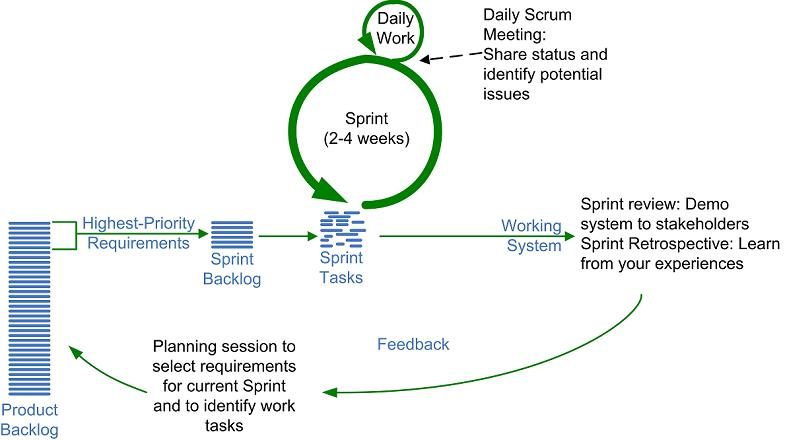
\includegraphics[width=\textwidth, keepaspectratio=true]{scrumsprint}
\caption{Agile software development poster \citep{scrumsprint}}
\label{scrumsprint}
\end{figure}

Figure \ref{scrumsprint} represents the different iterations a team of developers iterates through when using agile development methodology.

\begin{figure}[!htpb]
\centering
	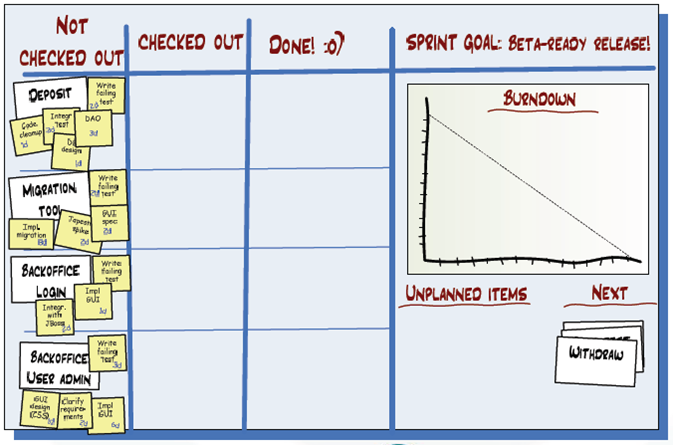
\includegraphics[width=0.8\textwidth]{scrumboard}
\caption{Example of scrum board \citep{scrumboard}}
\label{scrumboard}
\end{figure}

A scrum board as shown in Figure \ref{scrumboard}, is used for each milestone to show which issues have been started on and who is working on which feature. The chart to the right in the figure is a burn-down chart, stating how many hours the team has to work in order to complete on time.
